\section{Setup and electronics of the experiment} \label{sec:aufbau}

In this part of the report the general setup of the experiment will be shown.
Further, the steps performed to actually take the measurements in particular the electronics and signal conversion necessary will be discussed.

\subsection{Experimental Setup}

	The experiment consists of the actual detector, the electronics to shape the raw input signals and the data collection on a computer.

	\begin{figure}[ht]
		\centering
		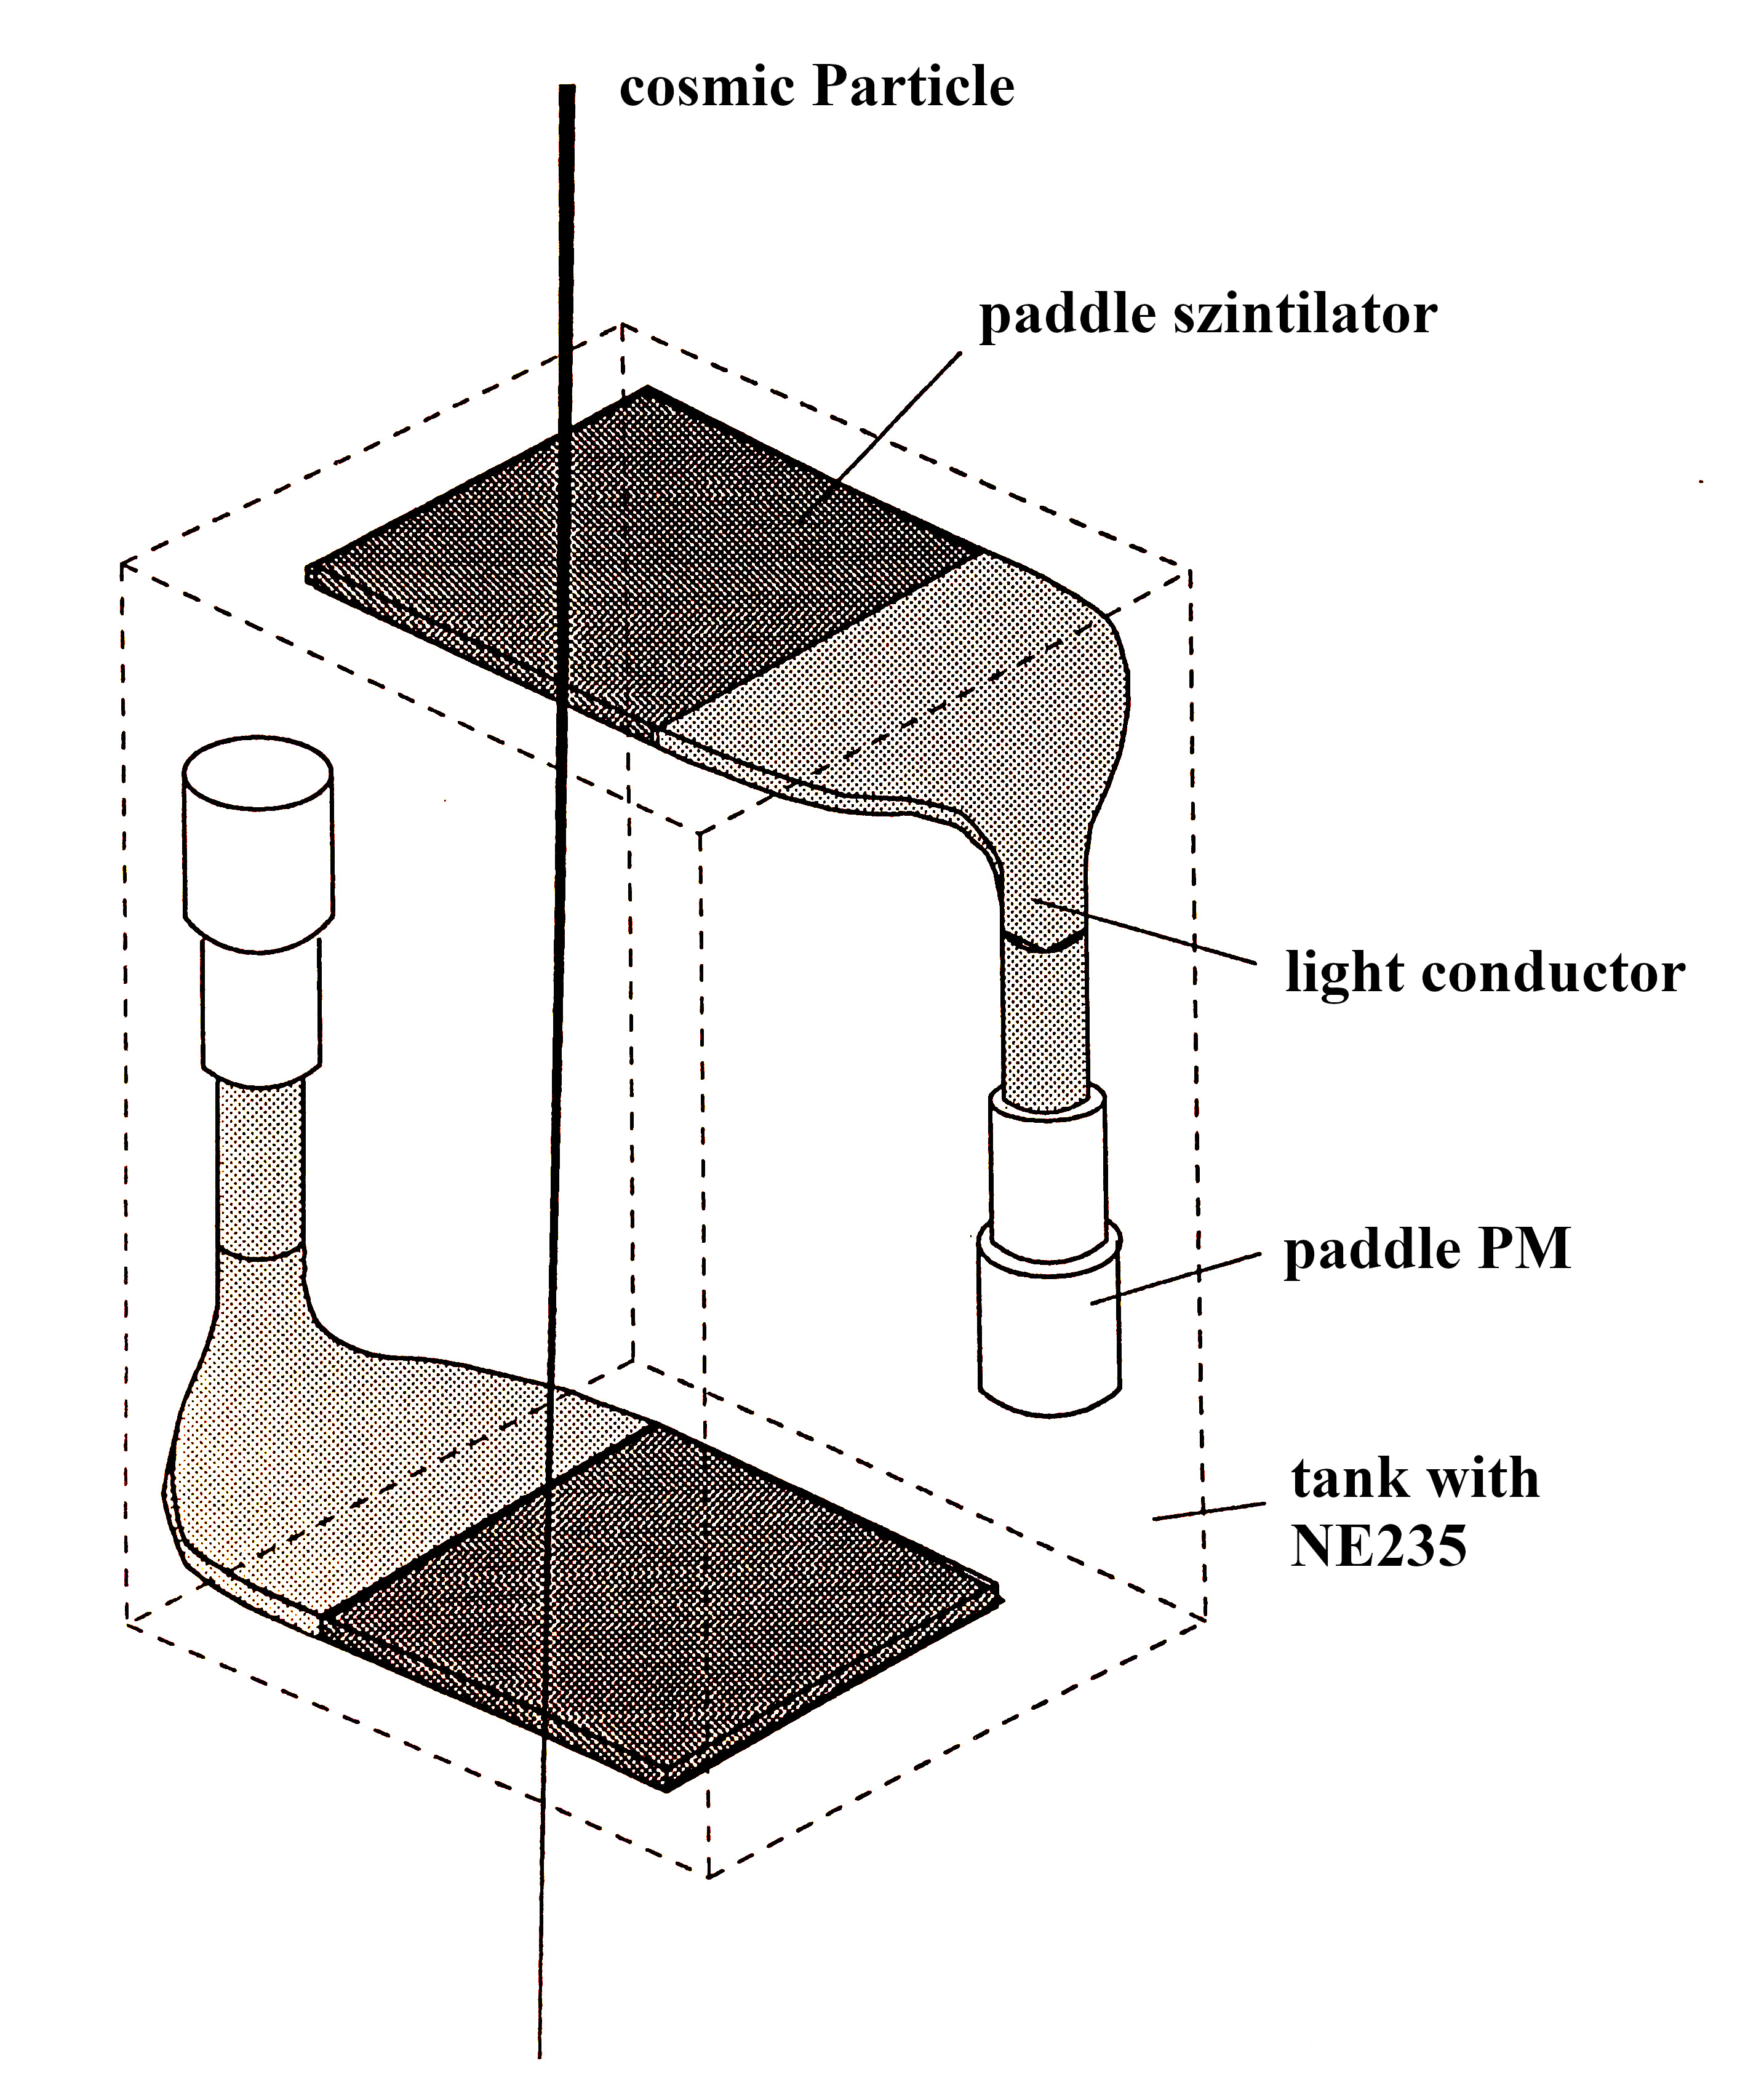
\includegraphics[width=0.5\textwidth]{img/aufbau.jpg}
		\caption{Concept of the detector. 
			The tank is filled with the liquid szintillator NE235.
			The paddles on both ends can determine the general angle of incident.
			The photo-multipliers of the tank itself are not shown.
			Taken from \cite{wwu}.}
		\label{fig:detector}
	\end{figure}
	
	The detector is made of a cuboid tank of size ($27 \times 27 \times 41$\,\si{\centi\meter\cubed}) filled with the liquid szintillator NE235, as shown in fig. (\ref{fig:detector}).
	To be able to measure the signal in the tank two photo-multipliers are extended on opposing corners of the detector.
	In the following, these are called the main photo-multipliers or PM's for short.
	Because of some electronic error in the HV unit only one of the PM's are actively used, as they are only used for slightly higher statistics.
	To be able to determine the general angle of incident, two szintillators with corresponding photo-multipliers are mounted on top and below the tank.
	Because of their shape, these are called paddles.
	They have a volume of ($190 \times 190 \times 6$\,\si{\milli\meter\cubed}) and are positioned \SI{550}{\milli\meter} from the core of the tank.
	The geometry of the paddles are the main source of uncertainty for the zenith angle measurement.
	
\subsection{Electronics}
	
	The electronics in this experiment is used to extract different information of the $\mu$-incident.
	While the specific electronics used in both measurements vary greatly and are explained later, some parts are essential for the general data processing and will be discussed first.
	
	The szintillators are able to convert incoming particles with high energies into a set of low energy photons.
	Because the energy of those photons is constant and determined by material used as a szintillator, the amount of created photons is also proportional to the energy deposited in the szintillator.
	A photo-multiplier-tube is then used to convert these low energy photons to electrons and through a cascade of dynodes deliver a current or charge, which is itself proportional to the deposited energy.
	For more information about szintillators and photo-multiplier-tubes one may read \cite{leo1994techniques}, chapter 7 to 9.
	
	The voltage for the photo-multipliers can be tuned using two HV-controllers with two HV-channels each.
	Both paddles should be operated at \SI{-1800}{\volt} and the PM's at \SI{-1000}{\volt} and \SI{-973}{\volt} respectively.
	One HV-unit was unable to deliver a voltage higher than approximately \SI{400}{\volt} and thus the second PM could not be used in the measurements.
	All photo-multipliers are connected to a pre-amplifier first.
	These will enhance the signal in strength and form for further processing and output a linearly dependent uni-polar signal.
	Normally the main PM's are combined through the logical or linear FI/FO unit for higher statistics, but in our case only one PM could be operated, so we connected the output of the pre-amplifier directly into the following unit.
	
	To be able to collect any data an analog-to-digital-converter (ADC) is used.
	It has a signal and a gate input and is connected to a computer with the corresponding software for data collection and management.
	The gate input is used to filter out unwanted signals and the ADC is only collecting data, while the gate is provided with a positive logical signal.
	Whenever the ADC is given a valid signal, it will sort it into one of 8192 channels, corresponding to the amplitude of the signal.
	For further analysis the channels have to be calibrated in a way.
	It is often assumed, that the correlation between amplitude and channel-number is linear, so only two calibration points are needed.
	
\subsubsection{Lifetime-Measurement}
	
	\begin{figure}[ht]
		\centering
		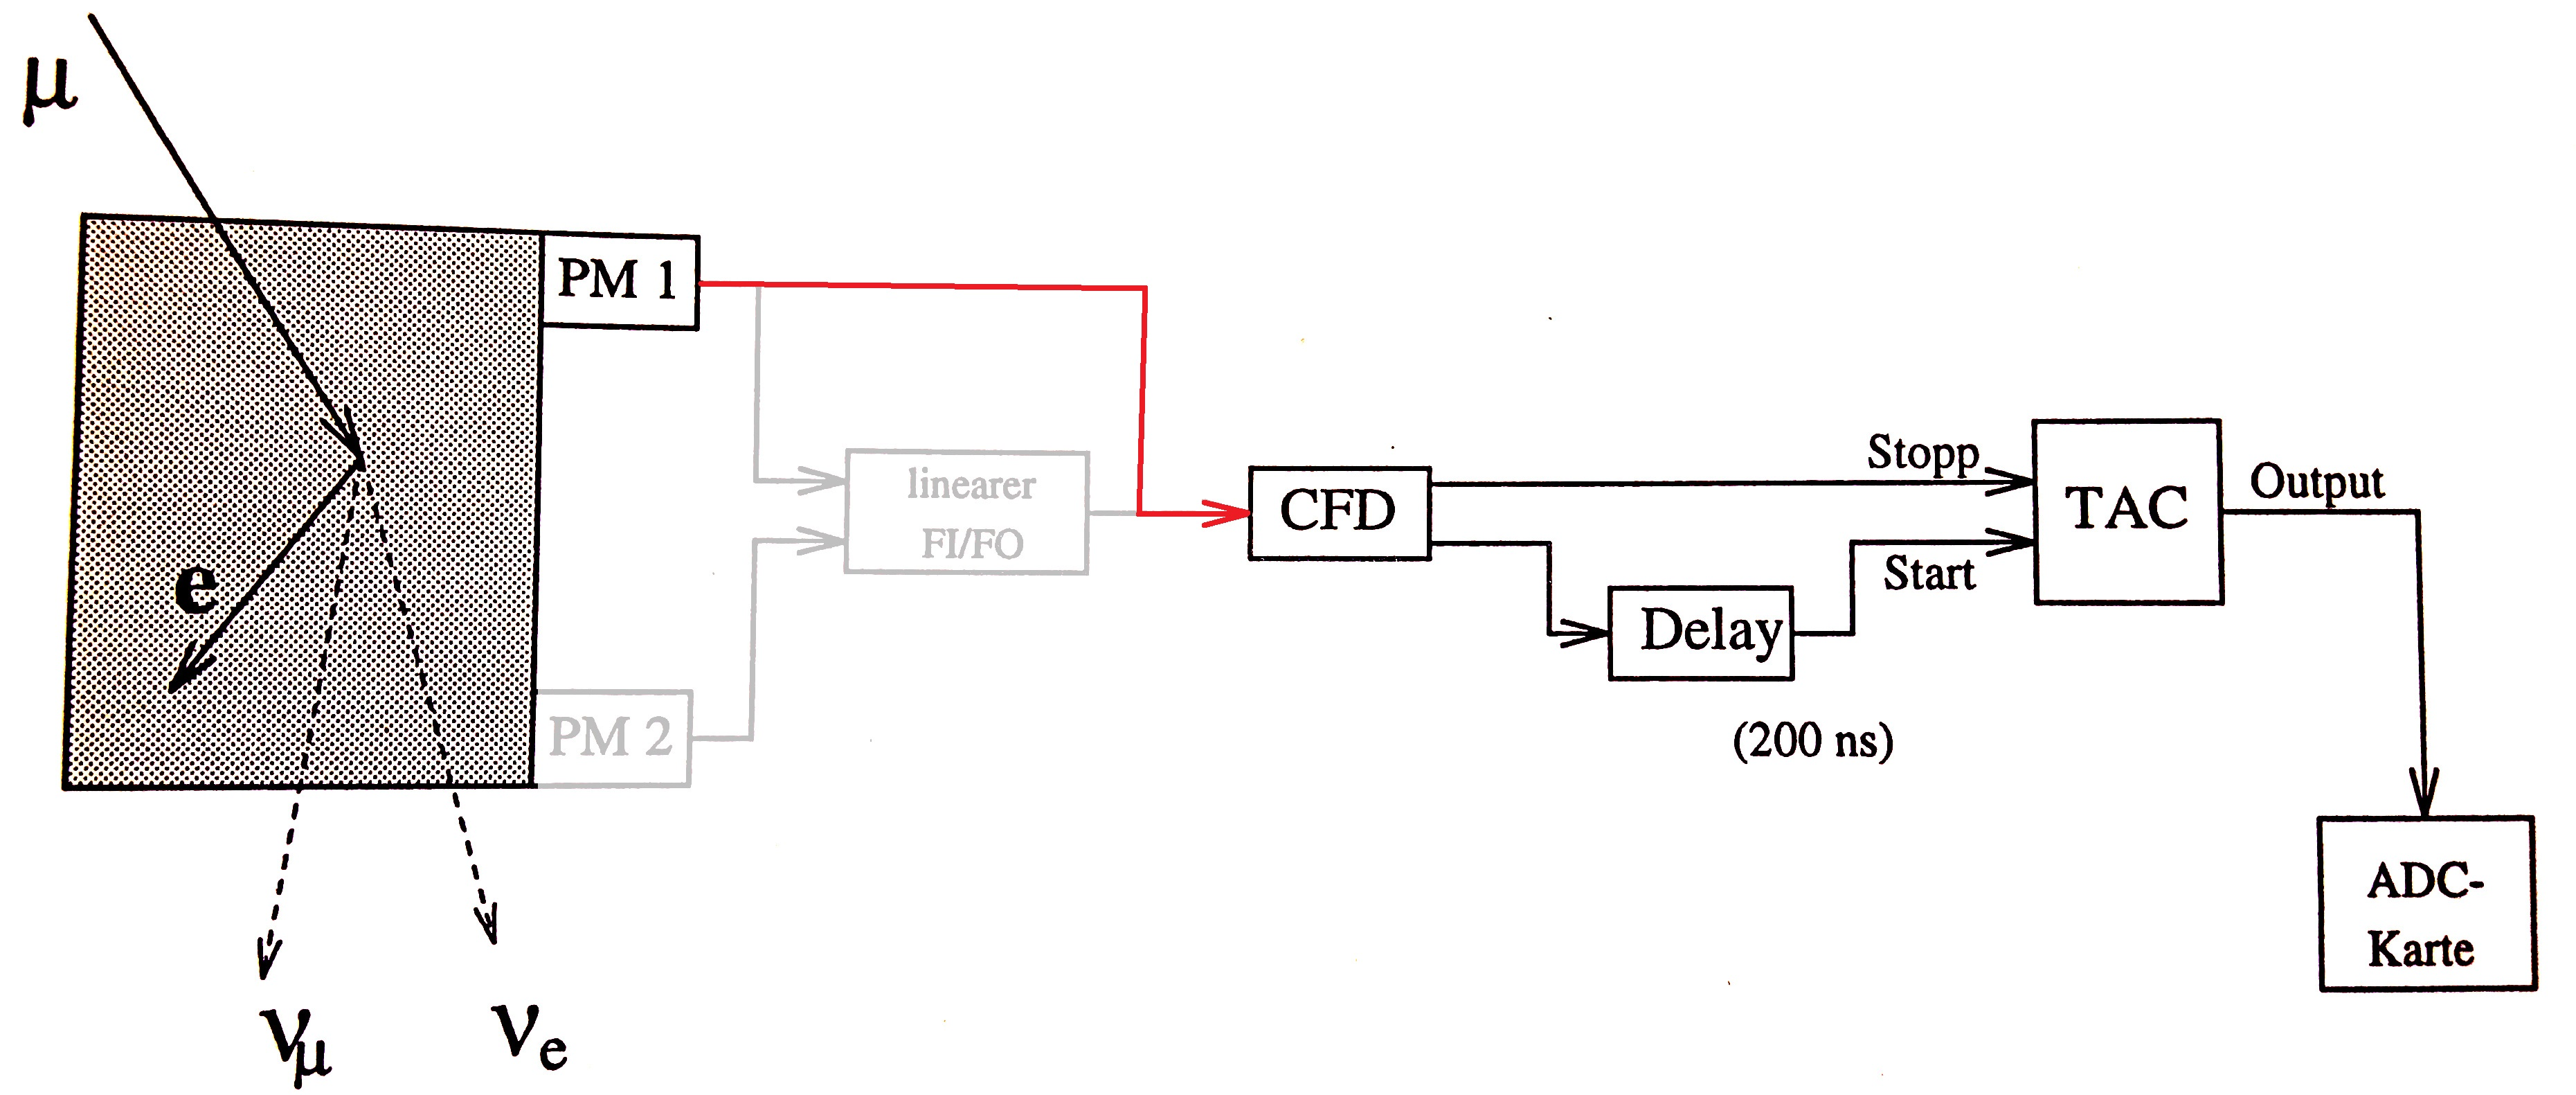
\includegraphics[width=0.7\textwidth]{img/lebensdauer.jpg}
		\caption{Electronics for the lifetime measurement.
			An incoming event is measured by the PM's and starts the TAC unit after a short delay.
			The following signal comes from the electron and stops the TAC unit.
			The difference in time of both signals will be collected by the ADC.
			Taken from \cite{wwu} and edited.
		}
		\label{fig:electronics_lifetime}
	\end{figure}

	To be able to measure the lifetime of a decaying $\mu$, one needs to measure the difference of the incoming $\mu$ and the outgoing $e$ very precisely.
	To achieve high precision a snap-off-timing-discriminator (CFD) is used in conjunction with a time-to-amplitude-converter (TAC), as shown in fig. (\ref{fig:electronics_lifetime}).
	The TAC is measuring the time between a starting and a stopping trigger and outputs a single signal, which amplitude is linearly dependent on this time difference.
	If no stopping trigger is supplied within a pre-defined reset time, the TAC will output no signal at all.
	For this measurement the reset time is set to \SI{20}{\micro\second}, as about 99.97\,\% of all captured $\mu$ will decay in this time period.

	\begin{figure}[ht]
		\centering
		\begin{subfigure}{0.32\textwidth}
			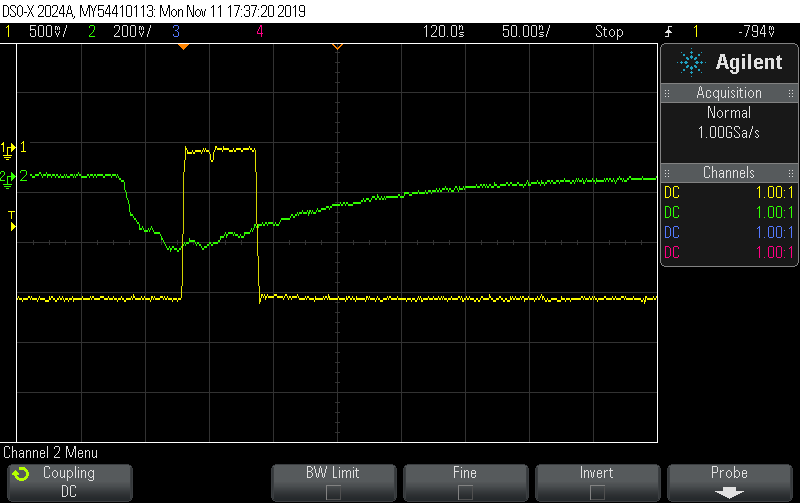
\includegraphics[width=\textwidth]{img/Lebensdauer/scope_3.png}
			\subcaption{}		
		\end{subfigure}
		\begin{subfigure}{0.32\textwidth}
			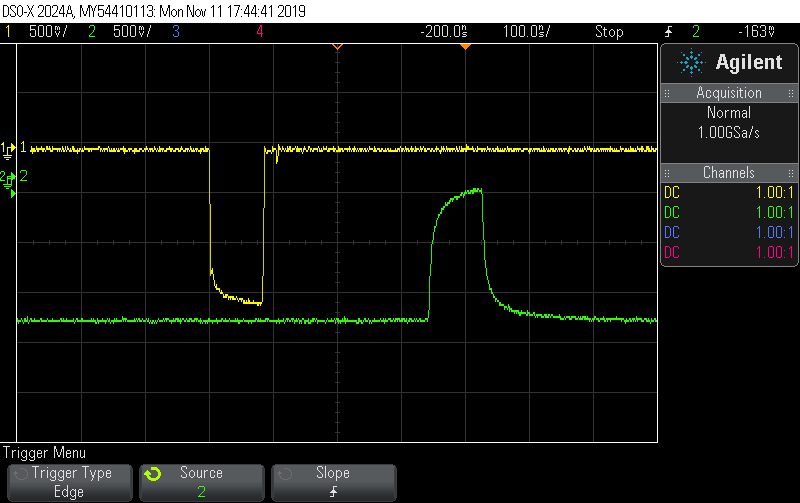
\includegraphics[width=\textwidth]{img/Lebensdauer/scope_4.png}
			\subcaption{}
		\end{subfigure}
		\begin{subfigure}{0.32\textwidth}
			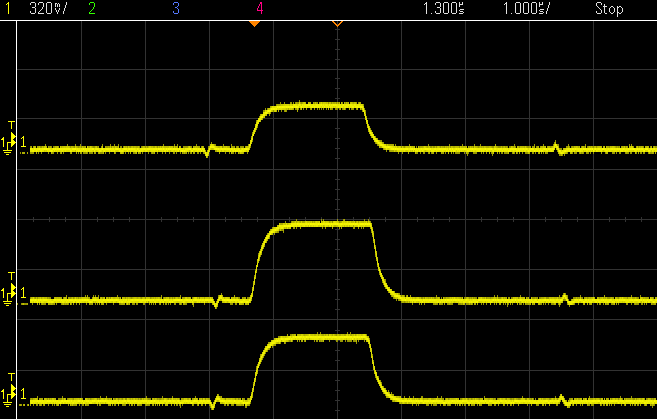
\includegraphics[width=\textwidth]{img/Lebensdauer/scope_5.png}
			\subcaption{}
		\end{subfigure}
		
		\caption{Signal shapes of the lifetime-measurement displayed on an oscilloscope.
			In (a) the original signal from the main PM (green) and the discrete logical signal from the CFD (yellow) are shown. One can clearly see the fast rising time and the logical operating voltage of \SI{1.5}{\volt}.
			(b) depicts the delay of the signal with the long cable. The actual delay of the cable is about \SI{350}{\nano\second}.
			(c) is a composition of different outputs of the TAC. The amplitudes of those signals vary, while their length is constant.
		}
		\label{fig:signal_lifetime}
	\end{figure}

	The incoming $\mu$ is generating a short signal and is stopped inside the tank.
	The signal is enhanced by the CFD and delayed by approximately \SI{350}{\nano\second}\footnote{In the instructions a delay of \SI{200}{\nano\second} is given, but after comparing the signals with each other as shown in fig. (\ref{fig:signal_lifetime}, b) the actual time delay has been corrected.} to not instantly trigger the TAC.
	A long cable is used to delay the signal with needed precision.
	Because the signal is much shorter than the delay, the stopping trigger is long gone, when the starting trigger is supplied.
	
	After the decay of the $\mu$, the resulting $e$ is causing the next signal and stopping the TAC.
	Because of the delay-cable the TAC is actually starting the next measurement, but no further signals are detected, so the TAC is not outputting any signal.
	The resulting signal from the TAC is put into the ADC and is proportional to the time difference between incoming $\mu$ and outgoing $e$.
	The transformation of the signals is shown in fig. (\ref{fig:signal_lifetime}).
	
\subsubsection{Angle-Measurement}

	\begin{figure}[ht]
		\centering
		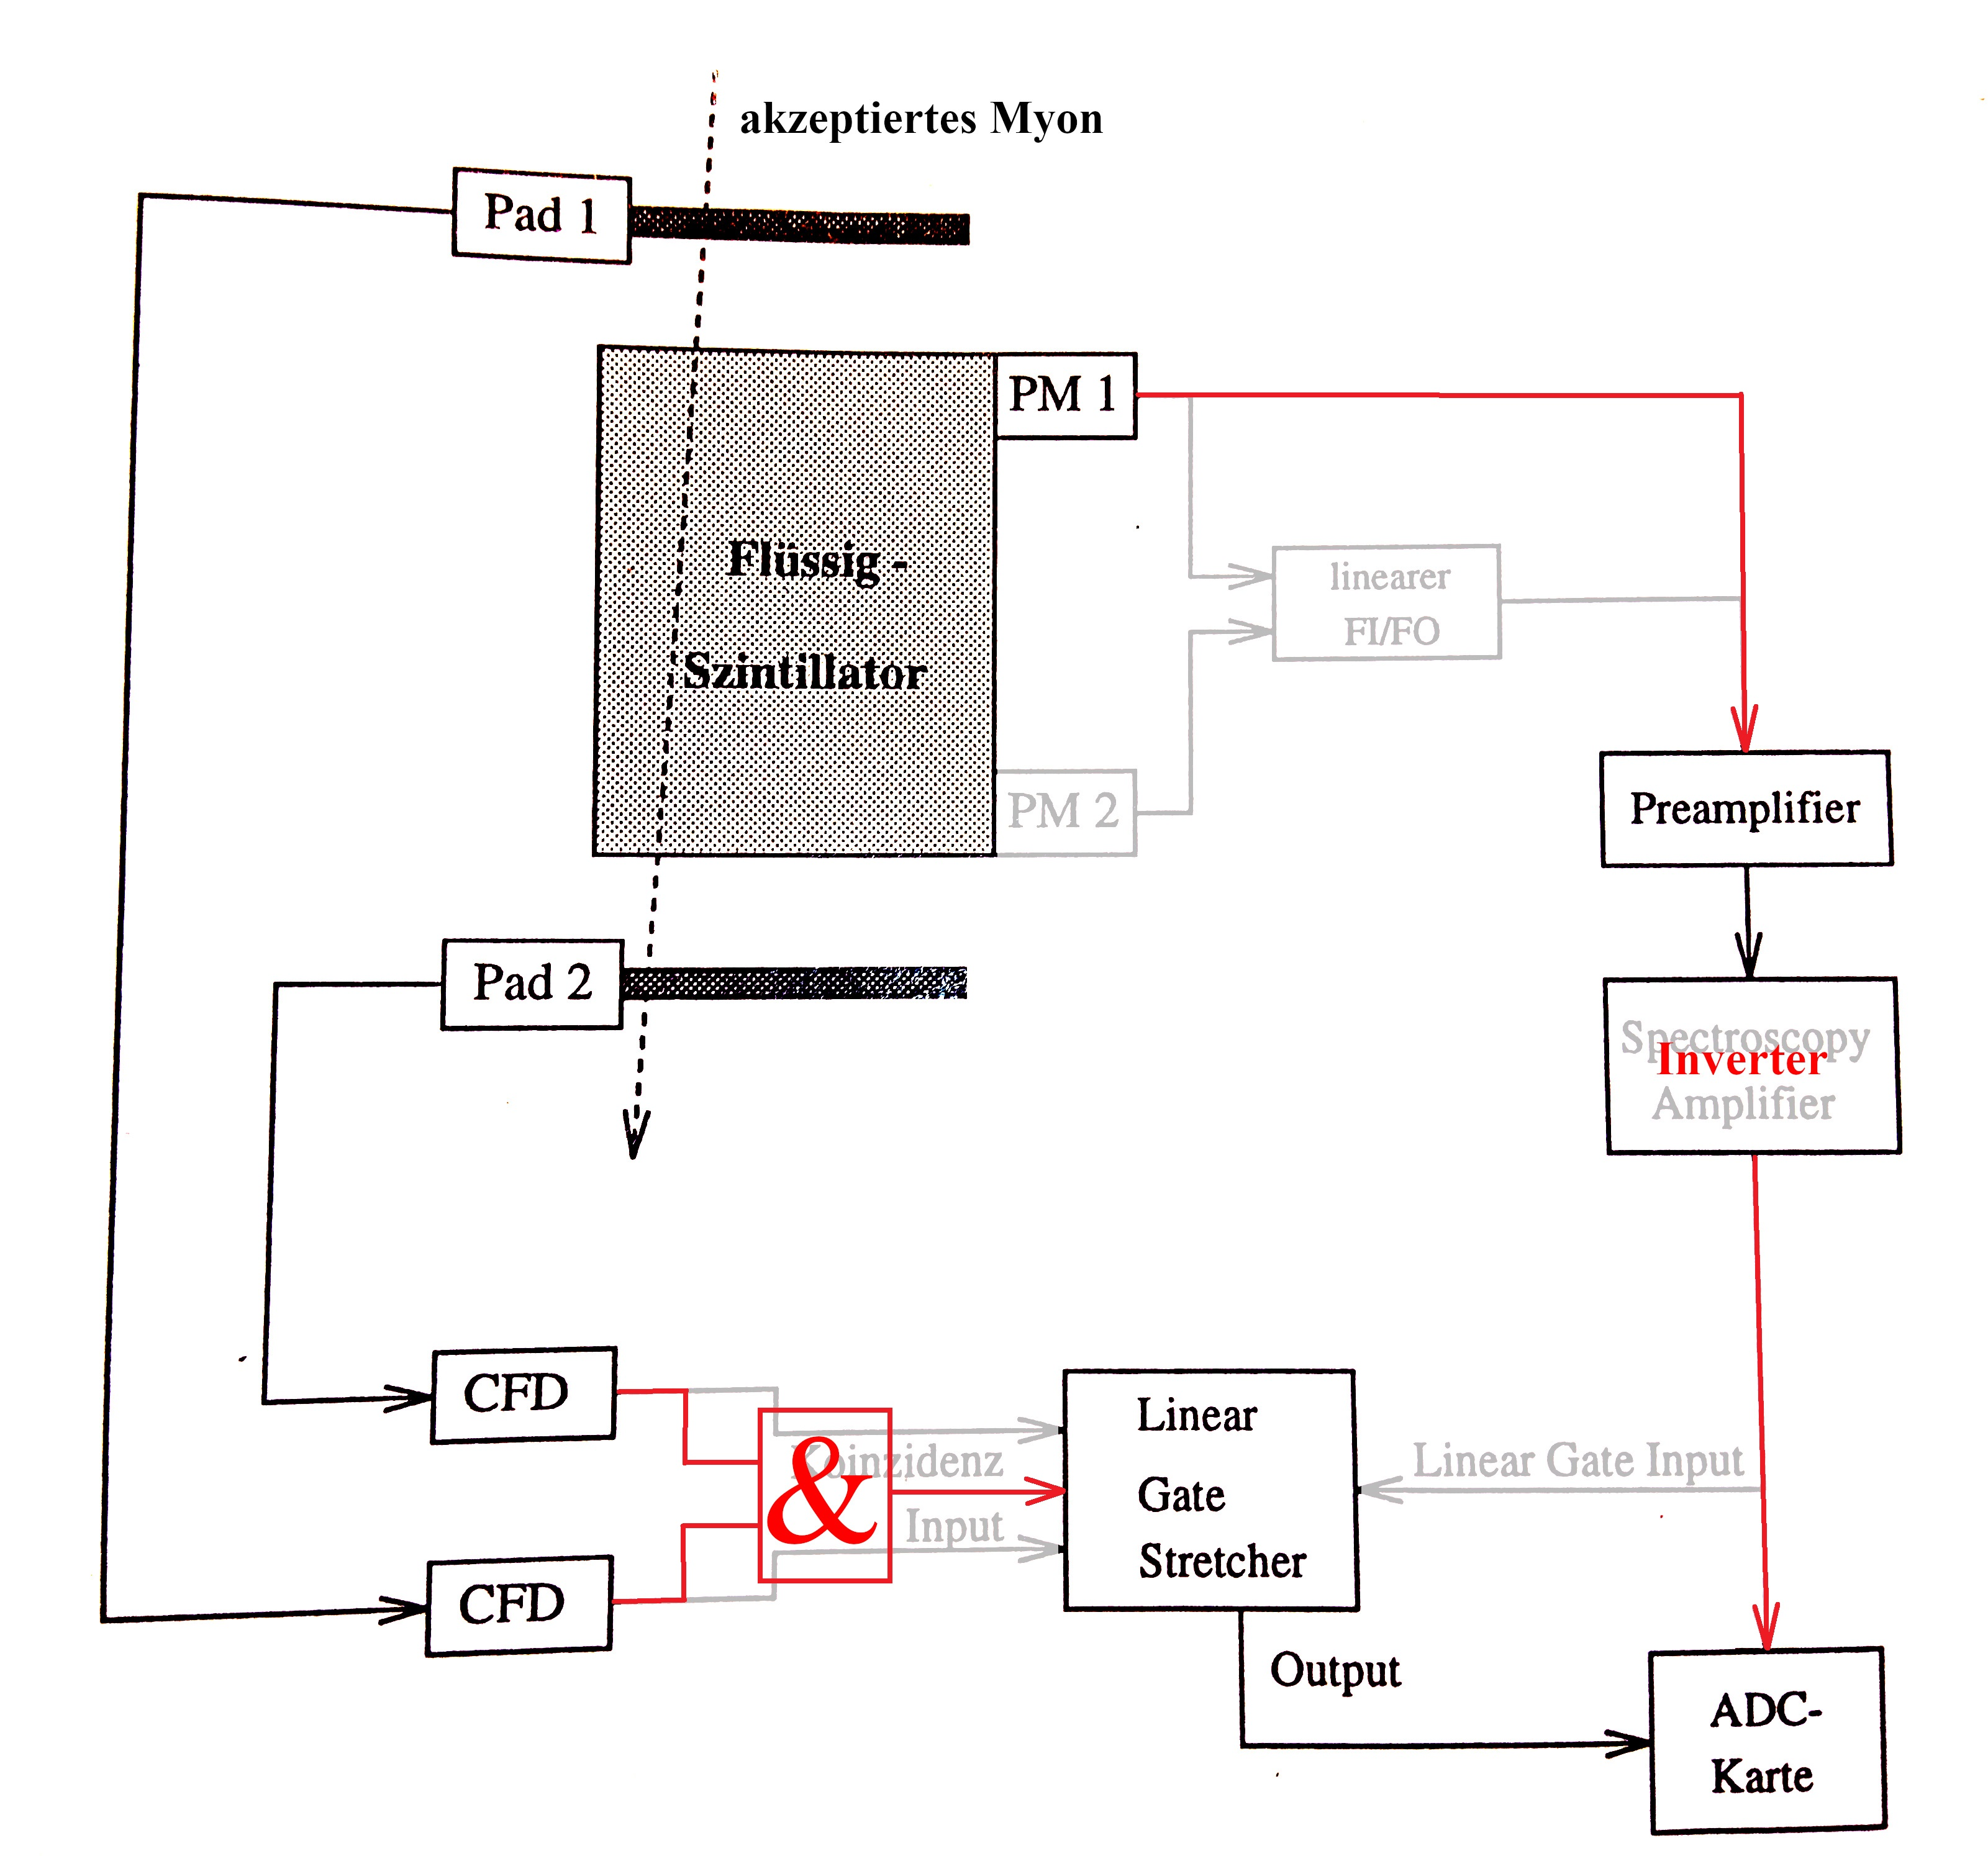
\includegraphics[width=0.6\textwidth]{img/winkel.jpg}
		\caption{Electronics for the angle-measurement.
				The signal from the main PM is only collected by the ADC, when the $\mu$ is traversing both paddles.
				To ensure the correct data collection, the coincidence signal is stretched, while the energy signal is delayed through a long cable.
			}
		\label{fig:electronics_angle}
	\end{figure}

	To be able to make any statement about the correlation between the intensity and the zenith angle of incoming $\mu$, one has to be able to determine, if a $\mu$ is coming from a specific angle of incident.
	In this experiment the paddles are used as a gate trigger for the ADC and an event is only collected, when both paddles are simultaneously activated.
	
	\begin{figure}[ht]
		\centering
		\begin{subfigure}{0.32\textwidth}
			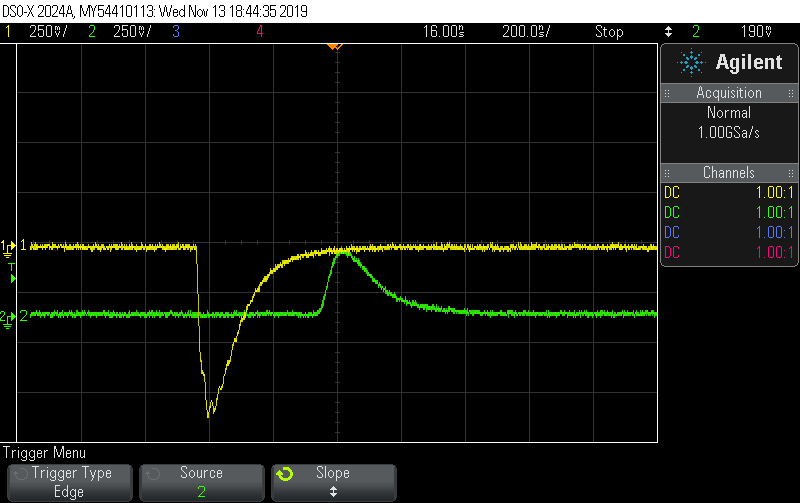
\includegraphics[width=\textwidth]{img/Winkel/scope_7.png}
			\subcaption{}		
		\end{subfigure}
		\begin{subfigure}{0.32\textwidth}
			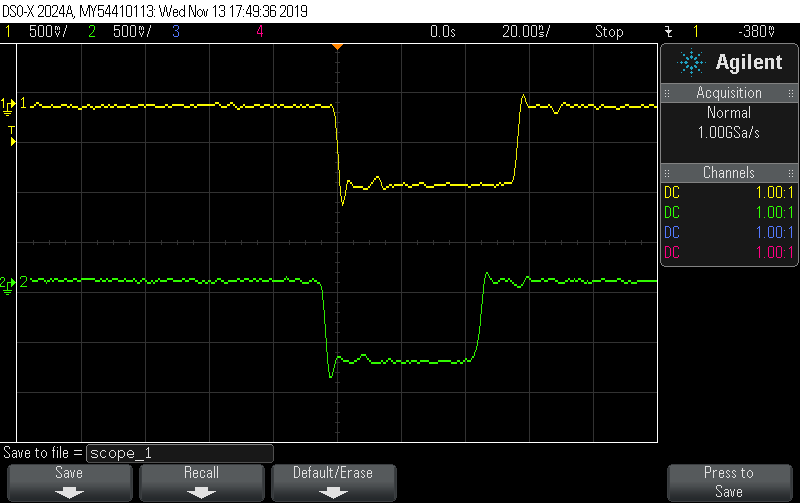
\includegraphics[width=\textwidth]{img/Winkel/scope_1.png}
			\subcaption{}
		\end{subfigure}
		\begin{subfigure}{0.32\textwidth}
			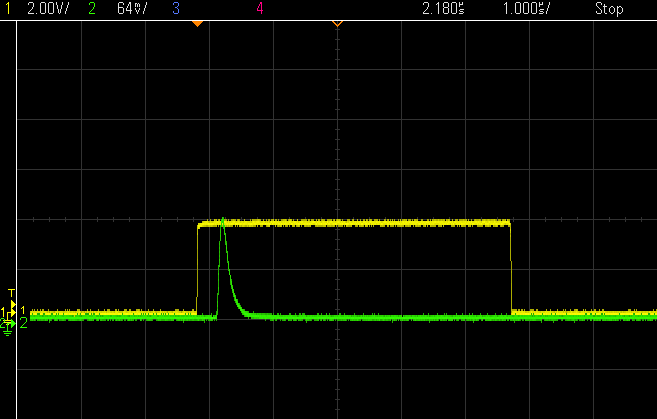
\includegraphics[width=\textwidth]{img/Winkel/scope_8.png}
			\subcaption{}
		\end{subfigure}
		
		\caption{Signal shapes of the angle-measurement displayed on an oscilloscope.
		(a) shows the signal output from one paddle (yellow) and the main PM (green) after it has been inverted.
		In (b) the coincidence between the two paddles is portrayed. The slight time difference of the two signals might be indicating, that the green paddle is the one on top of the detector.
		In (c) the final signals are depicted. The gate signal (yellow) opens the gate for a time frame long enough, so the actual energy signal (green) can be measured.
	}
		\label{fig:signal_angle}
	\end{figure}

	As shown in fig. (\ref{fig:electronics_angle}), the signals from the paddles are transformed into logical signals in the CFD.
	Afterwards they are combined in a coincidence-unit, so only if both paddles are activated at the same time, the output is true.
	Because the outgoing signal is just a very short peak, it is lengthened in a linear gate stretcher to about \SI{5}{\micro\second}.
	This signal is finally used, to trigger the gate input of the ADC.
	The main signal for the ADC is provided by the main PM, after it is amplified and inverted and is proportional to the energy of the incoming $\mu$.
	To make sure, that the signal is inside the time frame opened by the gate input, the signal is delayed by \SI{200}{\nano\second} with a long cable.
	The signal transformation of selected units can be seen in fig. (\ref{fig:signal_angle}).
	
\subsection{Operation}

	In case of the measurement of the $\mu$-lifetime, the ADC has to be calibrated.
	For this a time-calibrator (TC) was used and connected to the inputs of the TAC.
	The binned data is showing a regular set of peaks with defined distance to each other.
	Now the experiment has been assembled as described above and been run for two days to improve statistics.
	
	For the angle-measurement no calibration has to be done, as no quantitative value has to be gained from the diagram itself.
	So the second experiment has been assembled as stated above and been run for different zenith angles.
	The angles of \SIlist{0;30;45}{\degree} have been meassured for one day.
	Because the flux of incoming $\mu$ is greatly reduced for high zenith angles, the angle of \SI{75}{\degree} has been measured for two days in a row.
	
%zenith angle uncertainty given by $\Delta\Theta = \arctan \left( \frac{b}{a} \right)$, where $a = \SI{550}{\milli\meter}$ the distance of the paddles from the center of the tank and $b = \SI{190}{\milli\meter}$ the length of the paddles.

%Lebensdauer/Winkel
%- Schaltplan
%- Elektronik
%- Signalverarbeitung
%
%Lebensdauer
%- Detektoraufbau
% - Szintillator
% - Photomultiplier
% - Vorverstärker
% - Diskriminator
% - Or-Gate
% - ADC
